\documentclass[12pt]{article}

%-----------------------------------------------------------
% PACKAGES
\usepackage[a4paper, margin=1in]{geometry}
\usepackage{graphicx}
\usepackage{array}
\usepackage{xcolor}
\usepackage{tikz}
\usepackage{setspace}
\usepackage{hyperref} % <-- added

%-----------------------------------------------------------
\begin{document}

\begin{titlepage}

%-----------------------------------------------------------
% TOP BAND
\begin{tikzpicture}[remember picture,overlay]
\fill[blue!10] 
(current page.north west) 
rectangle ([yshift=-2cm]current page.north east);
\end{tikzpicture}

\vspace{1.2cm}

%-----------------------------------------------------------
% LOGOS
\noindent
\begin{minipage}[c]{0.5\textwidth}
\fbox{
\begin{minipage}[c][2.5cm][c]{4cm}
\centering
\small Company Logo
\end{minipage}
}
\end{minipage}
\begin{minipage}[c]{0.5\textwidth}
    \raggedleft
\end{minipage}

\vspace{0.6cm}
\noindent\rule{\textwidth}{0.5pt}

\vspace{1.2cm}

%-----------------------------------------------------------
% TITLE BLOCK
\centering

{\Large \bfseries Bridge Life Cycle Cost Analysis Report}

\vspace{1cm}

{\large \textit{Prepared using 3psLCCA}}\\[0.2cm]
{\small \href{https://osdag.iitb.ac.in/3pslcca}{osdag.iitb.ac.in/3pslcca}}

\vspace{1.6cm}

%-----------------------------------------------------------
% PROJECT INFORMATION (BOX STYLE)
\noindent
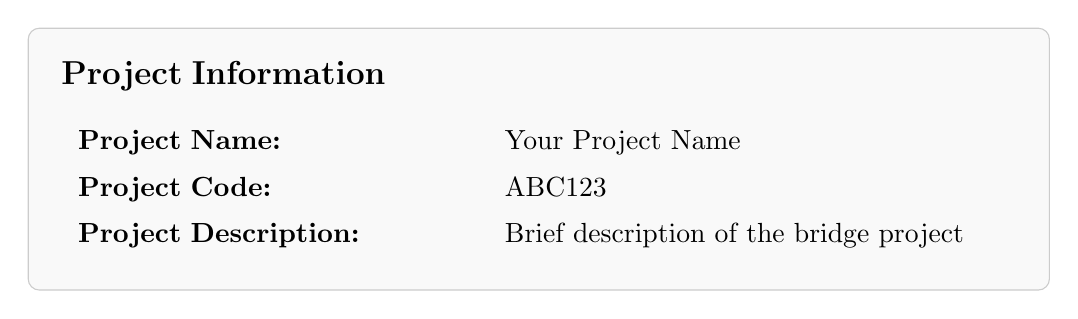
\begin{tikzpicture}
\node[draw=gray!40, fill=gray!5, rounded corners, inner sep=12pt, text width=\textwidth] {
\textbf{\large Project Information}

\vspace{3mm}

\renewcommand{\arraystretch}{1.4}
\begin{tabular}{p{5cm} p{9.5cm}}
\textbf{Project Name:} & Your Project Name \\
\textbf{Project Code:} & ABC123 \\
\textbf{Project Description:} & Brief description of the bridge project \\
\end{tabular}
};
\end{tikzpicture}

\vfill

%-----------------------------------------------------------
% EVALUATION & REVIEW BLOCK
\noindent
\begin{minipage}[t]{0.48\textwidth}
\textbf{\large Evaluated By}

\vspace{0.3cm}

\renewcommand{\arraystretch}{1.3}
\begin{tabular}{p{2.7cm} p{5.5cm}}
\textbf{Name:} & John Doe \\
% \textbf{Designation:} & Role \\
\textbf{Organization:} & Organization Name \\
\textbf{Address:} & Full Address Line \\
\textbf{Email:} & example@email.com \\
\textbf{Phone:} & +91-XXXXXXXXXX \\
\end{tabular}

\vspace{1.5cm}

{\centering
\rule{0.7\textwidth}{0.4pt} \\[-0.1cm]
\small Signature
\par}

\end{minipage}
\hfill
\begin{minipage}[t]{0.48\textwidth}
\textbf{\large Reviewed By}

\vspace{0.3cm}

\renewcommand{\arraystretch}{1.3}
\begin{tabular}{p{3cm} p{5.5cm}}
\textbf{Name:} & \\
% \textbf{Designation:} & \\
\textbf{Organization:} & \\
\textbf{Address:} & \\
\textbf{Email:} & \\
\textbf{Phone:} & \\
\end{tabular}

\vspace{1.5cm}

{\centering
\rule{0.7\textwidth}{0.4pt} \\[-0.1cm]
\small Signature
\par}

\end{minipage}

\vspace{1.2cm}


%-----------------------------------------------------------
% FOOTER
\vspace{0.5cm}

{\raggedright
\small
\textcolor{gray}{
Generated using 3psLCCA. The software is provided without any warranty, express or implied.\\
The life cycle cost analysis (LCCA) results depend on user-provided inputs. 
The evaluating agency is solely responsible for the accuracy of the input data and for any use of the results.
}
\par}

\end{titlepage}

\end{document}